\documentclass{article}
\usepackage[utf8]{inputenc}

\usepackage{natbib}
\usepackage{graphicx}
\usepackage{imakeidx}
\usepackage{caption}
\usepackage{listings}

\usepackage{hyperref}
\hypersetup{
    colorlinks=true,
    linkcolor=blue,
    filecolor=magenta,      
    urlcolor=cyan,
}

%%%%%%%%%%%%%%%%%%%%%%%%%%%
%%        EDICION        %%
%%%%%%%%%%%%%%%%%%%%%%%%%%%

\usepackage{todonotes}

%%%%%%%%%%%%%%%%%%%%%%%%%%%

\graphicspath{ {images/} }
\makeindex


% Title data
\title{Control parental de accesos WiFi}
\author{Esteban Omelio Puentes Silveira}
\date{Mayo, 2017}

\begin{document}
\maketitle

%\begin{figure}[h!]
%    \centering
%        \includegraphics[scale=0.2]{logo_uvigo.png}
%        \caption*{Universidad de Vigo}
%        \label{fig:uvigo}
%\end{figure}

\clearpage

%%%%%%%%%%%%%%%%%%%%%%%%%%%%%%%%%%%
%% DEDICATORIA Y AGRADECIMIENTOS
%%%%%%%%%%%%%%%%%%%%%%%%%%%%%%%%%%%

\section{Dedicatoria}

\section{Agradecimientos}

\clearpage


%%%%%%%%%%%%%%%%%%%%%%%%%%%%%%%%%%%
%% ÍNDICE
%%%%%%%%%%%%%%%%%%%%%%%%%%%%%%%%%%%

\renewcommand\contentsname{Índice}
\tableofcontents
\printindex


%%%%%%%%%%%%%%%%%%%%%%%%%%%%%%%%%%%
%% CONTENIDO
%%%%%%%%%%%%%%%%%%%%%%%%%%%%%%%%%%%
\todo{preguntar Moncho dónde va la arquitectura y si la planificación va en la introducción y eso, comparado con la lógica y lo que tengo en el TFG de cacho}

\section{Introducción}
%haberá que incluír unha introdución ao problema e xustificación do
%traballo realizado. En caso de que o TFG integre ou desenvolva traballos feitos na
%actividade doutras materias da titulación, o/a estudante deberá especificar os devanditos
%traballos e materias nesta sección.*/


    \subsection{Objetivos}
    \todo{debería ser subsection?}
    % presentar o problema que se vai tratar, incluír o obxectivo principal e os
    % específicos, de ser o caso, do traballo presentado, indicando o alcance para cada un deles.

    \subsection{Resumen de la solución propuesta}
    \todo{debería ser subsection?}
    % indicarase a solución aportada para o problema
    % presentado. Deberase incluír aquí a metodoloxía empregada.

\section{Planificación y seguimiento}
% deberase incluír un diagrama de Gantt que amose tanto
% a planificación do traballo, coa súa distribución de fases e tarefas, e a súa comparación cos
% datos reais obtidos tras o desenvolvemento do traballo.

\section{Arquitectura y tecnologías}
% explicarase a arquitectura empregada para alcanzar os obxectivos propostos.

    \subsection{Arquitectura del sistema}

    \subsection{Tecnologías e integración de productos de terceros}
    % describiranse adecuadamente as tecnoloxías utilizadas para o desenvolvemento do traballo, así coma os diversos productos que non son da autoría do/da estudante, xustificando a súa utilización.

\section{Especificación y análisis de requisitos}
% describiranse os requisitos necesarios, tanto funcionais como non funcionais. Incluiranse os aspectos máis relevantes correspondentes á análise do traballo realizado.
% IEEE830

    \subsection{Introducción}
    % En este apartado se detalla la Especificación de Requisitos Software, de ahora en

    % adelante ERS, del Sistema de Gestión Erasmus (EMS). La ERS facilita el mecanismo

    % apropiado para comprender lo que quiere el cliente, analizando necesidades, confirmando

    % su viabilidad, negociando una solución razonable, especificando la solución sin

    % ambigüedad, validando la especificación y gestionando los requisitos para que se

    % transformen en un sistema operacional.


    \subsection{Propósito}

    % El propósito es definir de manera clara y precisa las funcionalidades, características

    % y restricciones técnicas del Sistema. Esta especificación será sometida a revisión a medida

    % que avance el Sistema para corroborar que se cumple con lo estrictamente establecido.


    \subsection{Ámbito del Sistema}

    % Actualmente, tanto el personal designado para empeñar las funciones de

    % coordinador Erasmus como la propia ORI no disponen de ningún sistema de manejo

    % documental online que facilite todo el proceso de solicitud y seguimiento del Erasmus. En

    % este apartado se especifican los requisitos necesarios para el desarrollo de una aplicación

    % informática, denominada por el nombre de EMS (Sistema de Gestión Erasmus), que agilice

    % el proceso de control y solicitud de plazas y requisitos específicos además de poder realizar

    % una asignación automática de destinos Erasmus, facilitando y agilizando la labor que esto

    % conlleva a cada coordinador.

    % Es importante resaltar que el sistema controlara y manejará toda la documentación que se

    % aplica en cada uno de los subprocesos de solicitud de la plaza y posteriormente de las

    % etapas diferenciadas de la estancia Erasmus, para que de esta manera sea mucho más

    % sencilla e intuitiva la manera de gestionar los destinos y toda la información y

    % documentación necesaria, lo cual beneficia a los usuarios al momento de emplear esta

    % aplicación.


    \subsection{Definiciones, Acrónimos y Abreviaturas}

    % • Definiciones:

    % EMS Palabra formada por las iniciales de Erasmus

    % Management System (Sistema de Gestión Erasmus).

    % • Acrónimos y abreviaturas:

    % ERS Especificación de Requisitos Software

    % RFXXX El estándar seguido para la especificación del

    % identificador de cada requisito funcional se nombrará

    % de la siguiente forma:

    % - R = Requisito

    % - F = Funcional

    % - XXX = Secuencia de hasta tres dígitos que

    % servirá para la enumeración de cada requisito.

    % RNFXXX El estándar seguido para la especificación del

    % identificador de cada requisito no funcional se

    % nombrará de la siguiente forma:

    % - R = Requisito

    % - NF = No Funcional

    % - XXX = Secuencia de hasta tres dígitos que

    % servirá para la enumeración de cada requisito.

    % RIFXXX El estándar seguido para la especificación del

    % identificador de cada requisito no funcional se

    % nombrará de la siguiente forma:

    % - R = Requisito

    % - I = Interfaz

    % - XXX = Secuencia de hasta tres dígitos que

    % servirá para la enumeración de cada requisito.

    % MVC Modelo Vista Controlador


    \subsection{Referencias}

    % Los estándares, metodología y documentación que sirven de base para la

    % elaboración del Plan de Especificación de Requerimientos se hacen referencia a

    % continuación:

    % La Especificación de requerimientos del Software se ha diseñado basándose en normas

    % dadas por el estándar IEEE Recommended Practice for Software Requirents Specification

    % ANSI/IEEE 830, 1998.


    \subsection{Visión general del documento}

    % Este análisis de requisitos consta de tres apartados claramente diferenciados. En

    % primer lugar este primer punto proporciona una introducción y una visión general de la

    % ERS. El segundo apartado muestra la descripción general del sistema, consiguiendo así

    % conocer las principales funciones que realiza así como los datos, restricciones, supuestos y

    % dependencias que afectan a su desarrollo. Por último, en el tercer punto se definen de

    % manera detallada los requisitos necesarios para cumplir con todas las funciones del sistema.


    \subsection{Descripción general}

        \subsubsection{Perspectiva del producto}

        % Se trata de implementar una aplicación web para la gestión del proceso de petición,

        % asignación y envío de documentación antes, durante y al final de la estancia erasmus. EMS

        % no forma parte de ningún sistema mayor, es decir, es una aplicación totalmente

        % independiente del resto de sistemas, por lo que no hay que tener en cuenta en ningún

        % momento dicho aspecto.


        \subsubsection{Funciones del producto}

        % El sistema EMS permite la realización de las siguientes funciones:

        % • Gestionar usuarios (Administrador):

        % El sistema, que cuenta con tres tipos de usuario: administradores, coordinadores y

        % alumnos, permite las altas, bajas y modificaciones de los usuarios.

        % • Gestionar perfil (Administrador, Coordinador, Alumno):

        % Cada uno de los tres tipos diferentes de usuarios puede consultar y modificar su

        % perfil cuando deseen.

        % • Gestionar contrato de estudios (

        % El sistema, que cuenta con tres tipos de usuario: administradores, coordinadores y

        % alumnos, permite las altas, bajas y modificaciones de los usuarios. Cada uno de los tres

        % tipos diferentes de usuarios puede consultar y modificar su perfil cuando deseen.

        % • Gestionar plazas erasmus:

        % El sistema, que cuenta con tres tipos de usuario: administradores, coordinadores y

        % alumnos, permite las altas, bajas y modificaciones de los usuarios. Cada uno de los tres

        % tipos diferentes de usuarios puede consultar y modificar su perfil cuando deseen.

        % • Gestionar preinscripciones

        % El sistema, que cuenta con tres tipos de usuario: administradores, coordinadores y

        % alumnos, permite las altas, bajas y modificaciones de los usuarios. Cada uno de los tres

        % tipos diferentes de usuarios puede consultar y modificar su perfil cuando deseen.

        % • Gestionar documentación

        % El sistema, que cuenta con tres tipos de usuario: administradores, coordinadores y

        % alumnos, permite las altas, bajas y modificaciones de los usuarios. Cada uno de los tres

        % tipos diferentes de usuarios puede consultar y modificar su perfil cuando deseen.

        % 7.2.3. Características de los usuarios

        % Los usuarios de esta app web, que son entrenadores o bien deportistas que poseen

        % la tarjeta TDU o la tarjeta PEF, no encontrarán ningún problema a la hora de moverse por

        % la interfaz debido a que ésta es muy intuitiva y de fácil manejo.


        \subsubsection{Restricciones}

        % Una de las restricciones sobre el sistema es que éste debe adaptarse a los diferentes

        % dispositivos móviles, ya que el uso de estos aparatos está muy extendido en los gimnasios

        % últimamente. Además, el desarrollo de esta app debe realizarse únicamente con tecnologías

        % que no requieran de un pago previo para poder ser usadas.

        % Otra restricción se trata de la disponibilidad de ciertos servicios de cara al usuario mediante

        % un control de acceso, ya que dependiendo del tipo de usuario que acceda a esta app,

        % algunos servicios no serán visibles.


        \subsubsection{Suposiciones y dependencias}

        % El sistema de información EMS funciona independientemente, sin necesidades de

        % comunicarse con otros sistemas externos, por lo que no hay dependencias respecto de

        % otros sistemas.


        \subsubsection{Requisitos futuros}

        % En un futuro quizás se incluyan notificaciones a los clientes relacionadas con las actividades

        % deportivas del gimnasio. Dichas notificaciones podrían llevarse a cabo para avisar a los

        % clientes de la oferta de una nueva actividad o la cancelación de alguna sesión deportiva.


    \subsection{Requisitos específicos}

    % A continuación se presentan todos los requisitos que deberán ser realizados por el

    % sistema. Todos los requisitos aquí expuestos son importantes y han sido descritos teniendo

    % en cuenta el criterio de los usuarios:


        \subsubsection{Interfaces externas}

        % El sistema interactuará con el hardware de las tarjetas Deportiva Universitaria

        % (TDU) y tarjetas Ponte en Forma (PEF). **** REQUITOS DE INTERFAZ///DEFINIR

        % INTERFAZ EXTERNA DE HARDWARE COMO LLEGA LA INFORMACIÓN


        \subsubsection{Funciones}

        % • RF1- Gestionar usuarios (Administrador, Entrenador) RF1:

        % RF1.1- El sistema permitirá el registro de un usuario no registrado. Para ello se les

        % proporcionará un identificador de usuario y una contraseña. Se deberá almacenar nombre,

        % apellidos, foto, dirección, email, contraseña y tipo: Deportista, Entrenador o Usuario. Sólo

        % el administrador podrá editar el campo tipo de usuario y realizar el registro de un

        % Entrenador u otro Administrador en el sistema.

        % Los usuarios deportistas almacenarán además un subtipo: TDU (tarjeta deportiva

        % universitaria) y PEF (programa Ponte En Forma). Los entrenadores podrán administrar a

        % deportistas. Los administradores podrán administrar a todos los usuarios.

        % RF1.2- Los usuarios registrados podrán modificar los datos de su cuenta a través

        % del perfil de usuario.

        % RF1.3- Se permitirá la consulta de los datos de los usuarios registrados y del

        % administrador a través del perfil de usuario.

        % RF1.4- El administrador del sistema podrá eliminar aquellas cuentas de usuarios

        % que considere oportunas según sus criterios, a través de la vista de menú avanzado de

        % usuario.

        % RF1.5- Se visualizará la sección de perfil para usuarios registrados y administrador.

        % Además se permitirá el acceso a esta sesión para modificar o consultar los datos relativos a

        % sus cuentas.

        % 8

        % RF1.6- El acceso al sistema se realizará a través de la página de login en la que se

        % solicitarán el nombre de usuario y la contraseña.

        % RF1.7- El administrador del sistema dispondrá de un menú avanzado desde donde

        % podrá gestionar todas las cuentas registradas en el sistema. Para acceder a este menú bastará

        % con utilizar su login y contraseña.

        % • RF2- Consultar perfil (todos):

        % Se mostrará el nombre, apellidos, foto y dirección email.

        % • RF3- Consultar información pública (todos):

        % Se mostrará instalaciones, localización, contacto, actividades y horarios.

        % • RF4- Gestionar actividades (Entrenador, Administrador):

        % RF4.1- Sólo los usuarios de tipo Entrenador y el Administrador podrán realizar el

        % alta de una actividad en el sistema. Cada actividad incluye nombre, horario, entrenador

        % responsable, sesiones y tipo de actividad. Hay dos tipos de actividad: en grupo e

        % individuales.

        % RF4.2- Sólo los usuarios de tipo Entrenador y el Administrador podrán modificar

        % los datos de las actividades (nombre, horario, entrenador responsable, sesiones y tipo de

        % actividad).

        % RF4.3- Sólo los usuarios de tipo Entrenador y Administrador podrán eliminar las

        % actividades que consideren oportunas.

        % • RF5- Gestionar entrenamientos (Administrador, Entrenador):

        % Se entiende por entrenamiento la asignación de una o varias tablas a un deportista o

        % a un grupo de deportistas.

        % RF5.1- Sólo los usuarios de tipo Entrenador y el Administrador podrán realizar el

        % alta de un entrenamiento. Cada entrenamiento incluye nombre de la tabla, entrenador

        % responsable, varias actividades asociadas, tipo actividad: individual o en grupo, número de

        % plazas disponibles, deportistas reservados, lugar, horario, y sesiones.

        % RF5.2- Sólo los usuarios de tipo Entrenador y el Administrador podrán modificar

        % los datos de los entrenamientos (nombre de la tabla, entrenador responsable, varias

        % actividades asociadas, tipo actividad: individual o en grupo, número de plazas disponibles,

        % deportistas reservados, lugar, horario, tipo actividad: individual o en grupo, entrenador

        % responsable y sesiones).

        % RF5.3- Sólo los usuarios de tipo Entrenador y Administrador podrán eliminar los

        % entrenamientos que consideren oportunos.

        % • RF6- Gestionar plazas reservadas (Administrador, Entrenador):

        % RF6.2- Sólo los usuarios de tipo Entrenador y el Administrador podrán asignar

        % deportistas a entrenamientos.

        % RF6.3- Sólo los usuarios de tipo Entrenador y Administrador podrán eliminar

        % deportistas asociados a entrenamientos según su criterio.

        % • RF7- Control de asistencia (Deportista):

        % Entrenamientos a los que ha asistido el deportista y plazas libres en actividades

        % individuales o grupales

        % • RF8- Consultar entrenamientos (Deportista):

        % Se presentarán los entrenamientos a los que está asociado el deportista.

        % • RF9- Imprimir tabla de entrenamiento (Deportista):

        % Se presentarán los entrenamientos a los que esté asociado el deportista, incluyendo

        % ejercicios.

        % • RF10- Gestionar sesiones (Entrenador, Administrador):

        % RF10.1- Sólo los usuarios de tipo Entrenador y el Administrador podrán realizar el

        % alta de una sesión. Cada sesión incluye nombre, tipo y tabla de ejercicios. Hay tres tipos de

        % sesiones: muscular, cardio y estiramientos.

        % 9

        % RF10.2- Sólo los usuarios de tipo Entrenador y el Administrador podrán modificar

        % los datos de las sesiones (nombre, tipo y tabla de ejercicios).

        % RF10.3- Sólo los usuarios de tipo Entrenador y Administrador podrán eliminar las

        % sesiones que consideren oportunas.

        % • RF11- Gestionar tabla de ejercicios (Entrenador, Administrador):

        % RF11.1- Sólo los usuarios de tipo Entrenador y el Administrador podrán realizar el

        % alta de tabla de ejercicios. Cada tabla incluye varios ejercicios y tipo de tabla. Hay dos tipos

        % de tabla: estándar y personalizada. A cada tabla de ejercicio se le asignaran varios

        % deportistas. A los deportistas TDU se les asignará tablas estándar. A los deportistas PEF se

        % les asignará tablas personalizadas.

        % RF11.2- Sólo los usuarios de tipo Entrenador y el Administrador podrán modificar

        % los datos de las tablas de ejercicios (ejercicios y tipo de tabla).

        % RF11.3- Sólo los usuarios de tipo Entrenador y Administrador podrán eliminar las

        % tablas de ejercicios que consideren oportunas.

        % • RF12- Gestionar ejercicios (Entrenador, Administrador):

        % RF12.1- Sólo los usuarios de tipo Entrenador y el Administrador podrán realizar el

        % alta de ejercicios. Cada ejercicio incluye nombre, imagen, video, comentarios y tipo

        % (muscular, cardio o estiramiento). Los ejercicios en cada sesión deberán tener el mismo tipo

        % que la sesión: ejercicios musculares sólo en sesiones de tipo muscular, etc.

        % - Los ejercicios de tipo muscular tendrán repeticiones y carga.

        % - Los ejercicios de tipo cardio tendrán tiempo o distancia.

        % - Los ejercicios de tipo estiramiento tendrán repeticiones o tiempo.

        % RF12.2- Sólo los usuarios de tipo Entrenador y el Administrador podrán modificar

        % los datos de los ejercicios (nombre, imagen, video y tipo (muscular, cardio o estiramiento).).

        % RF12.3- Sólo los usuarios de tipo Entrenador y Administrador podrán eliminar los

        % ejercicios que consideren oportunas.

        % • RF13- Gestión de ejercicios realizados (Deportista):

        % RF13.1- Almacenamiento de los ejercicios asociados al deportista, y si han sido

        % realizados o están por realizar. El deportista podrá marcar los ejercicios por realizar como

        % ya realizados.

        % RF13.2- El deportista podrá consultar sus ejercicios asociados, realizados o por

        % realizar.

        % • RF14- Gestionar revisiones médico-deportivas (Entrenador, Administrador):

        % Sólo los usuarios de tipo Entrenador y el Administrador podrán realizar el alta de

        % las revisiones médico-deportivas. Cada revisión incluye lugar, horario y serán asignadas a

        % uno o más deportistas de tipo PEF.

        % • RF15- Consultar historial de entrenamientos (Deportista):

        % Consultar estadísticas de los entrenamientos.

        % • RF16- Consultar estadísticas (Entrenador, Administrador):

        % Se consultarán según deportista y en general para todo el sistema.

        % • RF17- Gestión de notificaciones (Entrenador, Administrador):

        % Se informará vía email de las notificaciones que sean de interés para los deportistas.


        \subsubsection{Requisitos de rendimiento}

        % El sistema deberá soportar el acceso de la administración, así como de los

        % entrenadores y deportistas situados fuera de las instalaciones. Como referencia, se

        % considerará un rendimiento aceptable si el 95% de las transacciones se realizan en menos

        % de un minuto. El 95% de las acciones en las que el deportista puede marcar su asistencia a

        % un ejercicio deberán completarse en menos de medio minuto, al ser especialmente

        % importantes.


        \subsubsection{Restricciones de Diseño}

        % En la restricción de diseño se tendrá en cuenta que la aplicación debe ser responsive para

        % adaptarse a dispositivos móviles ya que la mayoría de usuarios utilizarán su móvil mientras

        % están en el gimnasio y luego podrán consultarlo desde su pc en casa.


        \subsubsection{Atributos de Sistema}

        % • Fiabilidad: La aplicación pasará las pruebas estipuladas tanto en alpha como en beta

        % para asegurar la estabilidad en la versión 1.0.

        % • Seguridad: Se utilizará encriptado de contraseñas en el servidor y el montaje del

        % mismo en un CPD con todas las medidas de seguridad.

        % Además se cuenta con 3 tipos de usuarios con distintos permisos: administradores,

        % entrenadores y deportistas. También se tendrá una vista pública a la que puede acceder

        % cualquiera sin usuario.

        % • Mantenimiento: El mantenimiento de la aplicación se intentará hacer lo más

        % sencillo posible ya que se usará el MVC y cualquier cambio que se quiera realizar.

        % • Portabilidad: El sistema será fácilmente ejecutable y accesible desde web.


        \subsubsection{Otros requisitos}

        % No contaremos con otros requisitos en este proyecto por el momento.


\section{Diseño de software}
% (estático e dinámico) ou do hardware: indicaranse os aspectos máis relevantes correspondentes ao deseño do traballo realizado


\section{Gestión de datos e información}
% Xestión de datos e información: describiranse os métodos ou técnicas empregadas para xestionar tanto os datos coma o resto de información relevante.


\section{Pruebas llevadas a cabo}

% describiranse as probas realizadas aos distintos niveis para

% garantir o correcto funcionamento do software ou do hardware.

\todo{Requisitos mínimos}
\section{Manual técnico}
    \subsection{Requisitos mínimos}
        Para poder utilizar el sistema \textbf{Wifither} se debe cumplir un conjunto de requisitos, los cuáles están especificados a continuación.

        \todo{puntos}
        Equipo con una distrubución GNU/Linux para compilar paquete. Ubuntu como subsistema de Windows, BSD o MacOS no están oficialmente soportados, aunque suelen dar buenos resultados. Cygwin no está soportado debido al sistema de archivos que utiliza, que no es capaz de distinguir entre mayúsculas y minúsculas.

        Router con sistema operativo OpenWRT donde se ejecutará el servicio servidor.

        Dispositivo móvil con sistema operativo Android donde se instalará la aplicación cliente.

        Conexión a Internet tanto en el router como en el dispositivo móvil.

    \subsection{Compilar el paquete Wifither para OpenWRT}
        Aunque muchas de las dependencias necesarias suelen venir por defecto instaladas en diferentes sistemas operativos, es necesario que todas estén instaladas y funcionales. A continuación se muestra una tabla con las dependencias y el nombre de los paquetes en distribuciones \textit{Debian-like} \todo{style + modificar dependiendo de la tabla}

        \todo{debería poner toda la tabla? o quitar arch? o quitar todo?}
        %\begin{table}
            \begin{tabular}{|l|l|l|}
                \hline
                \textbf{Prerequisitos}  & \textbf{Debian}   & \textbf{Arch}             \\           
                \hline
                asciidoc                & asciidoc          & asciidoc                  \\
                GNU Bash                & bash              & bash                      \\
                GNU bc                  & bc                & bc                        \\
                GNU Binutils            & binutils          & binutils                  \\
                bzip2                   & bzip2             & bzip2                     \\
                fastjar                 & fastjar           & fastjar                   \\
                flex                    & flex              & flex                      \\
                git                     & git-core          & git                       \\
                GNU C++ Compiler        & g gcc-c           & -                         \\
                GNU C Compiler          & gcc               & gcc                       \\
                getopt                  & util-linux        & util-linux                \\
                GNU awk                 & gawk              & gawk                      \\
                gtk2.0-dev              & libgtk2.0-dev     & gtk2                      \\
                intltool-update         & intltool          & intltool                  \\
                jikes                   & jikespg           & -                         \\
                libz, libz-dev          & zlib1g-dev        & zlib                      \\
                Mercurial / hg          &                   & mercurial                 \\
                make                    & make              & make                      \\
                mkisofs                 & genisoimage       & cdrkit                    \\
                ncurses                 & libncurses5-dev   & ncurses                   \\
                openssl/ssl.h           & libssl-dev        & openssl                   \\
                patch                   & patch             & patch                     \\
                perl-ExtUtils-MakeMaker & perl-modules      & perl-extutils-makemaker   \\
                python2.6-dev           & python2.6-dev     & python2                   \\
                rsync                   & rsync             & rsync                     \\
                ruby                    & ruby              & ruby                      \\
                sdcc                    & sdcc              & sdcc                      \\
                subversion              & subversion        & subversion                \\
                unzip                   & unzip             & unzip                     \\
                GNU Wget                & wget              & wget                      \\
                xgettext                & gettext           & gettext                   \\
                xsltproc                & xsltproc          & libxslt                   \\
                zlib, zlib-static       & zlib1g-dev        & zlib                      \\
                \hline
            \end{tabular}
        %\end{table}

        Para instalar paquetes en distribuciones \textit{Debian-like} \todo{style} su utiliza el sieguiente comando.
        Es necesario que el usuario desde el que se ejecute el comando de instalación cuente con los permisos necesarios para llevar a cabo dicha acción.

        \todo{Estilos de estos códigos}
        \begin{lstlisting}[language=bash]
            $ apt-get install <paquete>
        \end{lstlisting}

        Varios paquetes pueden ser instalados a la vez utilizando el comando solo una vez.
        Ejemplo:

        \begin{lstlisting}[language=bash]
            $ apt-get install libncurses5-dev subversion gawk
        \end{lstlisting}

        Para preparar la compilación cruzada, descargar desde la página web oficial de OpenWRT \url{https://downloads.openwrt.org} el SDK correspondiente al modelo del dispositivo y la versión del sistema en el que se desea instalar el paquete. Una vez descargado, descomprimir el archivo y se copiar el código fuente dentro de la carpeta \textit{build} del SDK. Luego, desde la carpeta raíz del SDK, ejecutar los siguientes comandos para preparar las librerías que utiliza \textbf{Wifither}.

        \begin{lstlisting}[language=bash]
            $ ./scripts/feeds update
            $ ./scripts/feeds install uclibcxx
            $ ./scripts/feeds install libopenssl
        \end{lstlisting}

        \todo{arreglar}
        Una vez esté todo preparado, ejecutar el comando \textit{make} para llevar a cabo la compilación. El paquete resultante se almacena en \textit{SDK/bin/<modelo-router>/packages/base} con el nombre \textit{wifither_1_<modelo-router>.ipk}.


    \subsection{Instalación del servicio servidor} \todo{este nombre? demonio? servicio demonio? en el router?}
        En este apartado se explica cómo instalar el paquete \textit{.ipk} resultante de la compilación, en el router con OpwenWRT, cómo arrancar \todo{arrancar?} el servicio y cómo configurarlo para que inicie automáticamente cada vez que inicie el router.

        Primeramente se debe copiar el paquete al router donde se instalará, para ello se puede utilizar cualquier protocolo de red que permita la transferencia de archivos, en esta guía se explica cómo copiarlo mediante el uso de \textit{scp}. Para realizar este proceso, se debe especificar la ruta donde se encuetra el paquete, el usuario y equipo remoto al que se desea copiar, y la ruta donde se desea almacenar en ese equipo.

        \begin{lstlisting}[language=bash]
            $ scp <ruta-paquete> <usuario>@<equipo-remoto>:<ruta-almacenamiento>
        \end{lstlisting}

        Un ejemplo de la ejecución del comando:
        \begin{lstlisting}[language=bash]
            $ scp bin/brcm63xx/packages/base/wifither_1_brcm63xx.ipk root@192.168.0.4:/root/wifither
        \end{lstlisting}

        Una vez el paquete está en el router, este podrá ser instalado utilizando el gestor de paquetes de OpenWRT \textit{opkg}
        \begin{lstlisting}[language=bash]
            $ opkg install <ruta-paquete>
        \end{lstlisting}

        Para iniciar el servicio después de haberlo instalado se ejecutará \textit{wifiter} especificando el puerto en el que se desea recibir los paquetes y una contraseña que contenga al menos ocho caracteres.

        Ejemplo:
        \begin{lstlisting}[language=bash]
            $ wifither 4848 Potato12
        \end{lstlisting}

        Para configurar el equipo, de forma que Wifither siempre se inicie al arrancar el sistema, se debe editar el archivo \textit{/etc/rc.local} añadiendo la ejecución del servicio antes de la línea \textit{exit 0}

        \begin{lstlisting}[language=bash]
            # Put your custom commands here that should be executed once
            # the system init finished. By default this file does nothing.

            wifither 4848 Potato12

            exit 0
        \end{lstlisting}


    \subsection{Instalación de la aplicación móvil}
        Para realizar la instalación de la aplicación en el móvil existen dos opciones, utilizar la aplicación ya compilada \textit{.apk} o compilarla e instalarla directamente desde \textit{Android Studio}

        \subsubsection{Instalación del .apk}
            Es necesario que el archivo \textit{.apk} debe estar almacenado en el dispositivo móvil, para esto se puede conectar el dispositivo directamente al ordenador utilizando un cable USB.

            Para llevar a cabo la instalación debe estar activada la opción \textit{Fuentes desconocidas}, que se encuentra en el apartado \textit{Seguridad} de los ajustes del sistema Android. Esto hace que sea posible la instalación de aplicaciones que provengan de fuentes no oficiales.

            Una vez realizados los pasos anteriores, ir hasta la ubicación del archivo \textit{.apk}, pulsar sobre él y aceptar la instalación.

        \subsubsection{Compilar e instalar desde Android Studio}
            Para pider instalar aplicaciones utilizando este método es necesario que el dispositivo móvil esté conectado al ordenador mediante un cable USB y que esté activada la opción \textit{Depuración USB}, que se encuentra en el apartado \textit{Opciones de desarrollador} de los ajuste del sistema Android.
            \textbf{NOTA:} Las opciones de desarrollador están deshabilitadas por defecto en la mayoría de dispositivos Android, para habilitarla es necesario pulsar diez (10) veces sobre el \textit{Número de compilación}, que se encuentra en el apartado \textit{Acerca del dispositivo} de los ajuste del sistema Android.

            En la barra de menús de Android Studio, ir a \textit{File} y luego a la opción \textit{Open}, allí buscar y abrir la carpeta con el código fuente de la aplicación. Una vez haya cargado el proyecto, ir la opción \textit{Run 'app'} que se encuentra en el menú \textit{Run} y seleccionar el dispositivo.
            
            \textbf{NOTA:} Es importante aceptar en el dispositivo la clave RSA, esto permite que Android Studio pueda conectarse al dispositivo.

            Tras realizar los pasos anteriores, el código fuente debe haber quedado compilado, instalado y ejecutado en el dispositivo conectado.

    \todo{ddns, segundo router o router principal?}

    \subsection{Configuración de una VPN} \todo{cómo poner opcional?}
        En este apartado se explica la creación y configuración de una VPN en modo tunel entre el router y el dispositivo móvil mediante la utilización de OpenVPN. Esto paso es totalmente opcional ya que el sistema no lo necesita para su correcto funcionamiento, sin embargo, añade una capa de seguridad adicional que permite que todo el tráfico entre cliente y servido sea encriptado en origen y desencriptado en destino, por lo que nunca se conoce el contenido real de los paquetes enviados y no pueden ser replicados.

        \subsubsection{Creación de VPN en el router}
            Inicialmente se debe comprobar que los repositorios desde los que descargan los paquetes y librerías estén bien configurados en el router. Esto se puede observar en el archivo de configutación \textit{/etc/opkg/dist-feeds.conf}. Las rutas a los diferentes repocitorios dependerán de la versión del sistema y el modelo del router.

            Ejemplo:
            \url{https://downloads.openwrt.org}

            \begin{lstlisting}[language=bash]
                src/gz designated_driver http://downloads.openwrt.org/snapshots/trunk/brcm63xx/smp/packages/packages
                src/gz designated_base http://downloads.openwrt.org/snapshots/trunk/brcm63xx/smp/packages/base
                src/gz designated_packages http://downloads.openwrt.org/snapshots/trunk/brcm63xx/smp/packages/packages
                src/gz designated_luci http://downloads.openwrt.org/snapshots/trunk/brcm63xx/smp/packages/luci
                src/gz designated_routing http://downloads.openwrt.org/snapshots/trunk/brcm63xx/smp/packages/routing
                src/gz designated_telephony http://downloads.openwrt.org/snapshots/trunk/brcm63xx/smp/packages/telephony
                src/gz designated_management http://downloads.openwrt.org/snapshots/trunk/brcm63xx/smp/packages/management
            \end{lstlisting}
            
            Con los repositorios bien configurados, instalar \textit{openvpn-openssl} y \textit{openvpn-easy-rsa}
            
            \begin{lstlisting}[language=bash]
                $ opkg update
                $ opkg install openvpn-openssl openvpn-easy-rsa
            \end{lstlisting}

            \todo{Cómo funciona esto? Privado público?}
            A continuación se deben crear los certificados de seguridad para cliente y servidor. El siguiente código crea un certificado servidor con el nombre \textit{my-server} y un ccertificado cliente con el nombre \textit{my-client}. Se peuden crear tantos certificados clientes como sean necesarios ejecutando el mismo comando de creación \textit{build-key-pkcs12} varias veces especificando diferentes nombres.

            \begin{lstlisting}[language=bash]
                $ build-ca
                $ build-dh
                $ build-key-server <nombre-clave-servidor>
                $ build-key-pkcs12 <nombre-clave-cliente>
            \end{lstlisting}

            Una vez generadas las claves:
            
            \todo{punto}
                Copiar las perteneciantes al servidor servidor en el directorio \textit{/etc/openvpn}
            
                \begin{lstlisting}[language=bash]
                    $ cp /etc/easy-rsa/keys/ca.crt /etc/easy-rsa/keys/clave-servidor.* /etc/easy-rsa/keys/dh2048.pem /etc/openvpn
                \end{lstlisting}

                Copiar las pertenecientes al cliente en el dispositivo móvil mediante cualquier método disponible, puede ser a través de un dispositivo USB, un eMail, scp, etc.

                Ejemplo: Copiar las claves al equipo desde el que se compiló el paquete y conectar allí el dispositivo móvil
                \begin{lstlisting}[language=bash]
                    $ scp /etc/easy-rsa/keys/ca.crt /etc/easy-rsa/keys/clave-cliente.* root@192.168.0.100:/etc/openvpn
                \end{lstlisting}

            A continuación se muestran los comandos a ejecutar para la creación y configuración de una nueva red en el router por la que se realizarán las conexiones de la VPN y la configuración del cortafuegos correspondiente.

            \todo{enumerar}
            Crear la nueva interfaz de la VPN con el nombre vpn0
                
            \begin{lstlisting}[language=bash]
                $ uci set network.vpn0=interface
                $ uci set network.vpn0.ifname=tun0
                $ uci set network.vpn0.proto=none
                $ uci set network.vpn0.auto=1        
            \end{lstlisting}

            Configurar el cortafuegos para permitir conexiones entrantes al puerto \textit{1194} (puerto por defecto).

            \begin{lstlisting}[language=bash]
                $ uci set firewall.Allow_OpenVPN_Inbound=rule
                $ uci set firewall.Allow_OpenVPN_Inbound.target=ACCE  PT
                $ uci set firewall.Allow_OpenVPN_Inbound.src=*
                $ uci set firewall.Allow_OpenVPN_Inbound.proto=udp
                $ uci set firewall.Allow_OpenVPN_Inbound.dest_port=1194    
            \end{lstlisting}

            Crear nueva zona nombrada \textit{vpn} para la red vpn0. Esto permitirá las conexiones relacionadas con el tunel VPN, tanto entrantes como salientes.

            \begin{lstlisting}[language=bash]
                $ uci set firewall.vpn=zone
                $ uci set firewall.vpn.name=vpn
                $ uci set firewall.vpn.network=vpn0
                $ uci set firewall.vpn.input=ACCEPT
                $ uci set firewall.vpn.forward=REJECT
                $ uci set firewall.vpn.output=ACCEPT
                $ uci set firewall.vpn.masq=1   
            \end{lstlisting}

            Aplicar la nueva configuración.

            \begin{lstlisting}[language=bash]
                $ uci commit network
                $ /etc/init.d/network reload
                $ uci commit firewall
                $ /etc/init.d/firewall reload  
            \end{lstlisting}

            Configuración de OpenVPN:
            La configuración puede ser realizada medainte los archivos \textit{.conf} de OpenVPN o a través de la interfaz \textit{uci} de OpenWRT. En esta guía se indican los comandos a ejecutar para realizarlo mediante esta última opción.

            \begin{lstlisting}[language=bash]
                $ echo > /etc/config/openvpn
                $ uci set openvpn.myvpn=openvpn
                $ uci set openvpn.myvpn.enabled=1
                $ uci set openvpn.myvpn.verb=3
                $ uci set openvpn.myvpn.port=1194
                $ uci set openvpn.myvpn.proto=udp
                $ uci set openvpn.myvpn.dev=tun
                $ uci set openvpn.myvpn.server='10.8.0.0 255.255.255.0'
                $ uci set openvpn.myvpn.keepalive='10 120'
                $ uci set openvpn.myvpn.ca=/etc/openvpn/ca.crt
                $ uci set openvpn.myvpn.cert=/etc/openvpn/my-server.crt
                $ uci set openvpn.myvpn.key=/etc/openvpn/my-server.key
                $ uci set openvpn.myvpn.dh=/etc/openvpn/dh2048.pem
                $ uci commit openvpn
            \end{lstlisting}

            Iniciar OpenVPN
            \begin{lstlisting}[language=bash]
                $ /etc/init.d/openvpn enable
                $ /etc/init.d/openvpn start
            \end{lstlisting}

        \subsubsection{Conexión al la VPN desde dispositivo Android}
            Para establecer la conexión con la VPN se debe instalar la aplicación \textit{OpenVPN for Android} desde \textit{Google Play Store}
            
            \url{https://play.google.com/store/apps/details?id=de.blinkt.openvpn}

            Una vez instalada la aplicación, añadir un nuevo perfil desde la pestaña \textit{Profiles} presionando el botón \textit{Add Profile} y especificando un nombre. Después de realizar el paso anterior, en la pestaña \textit{Basic}, seleccionar \textit{PKCS12 File} como el tipo de autenticación a utilizar, luego presionar el botón \textit{Select...} de la parte superior y buscar en el almacenamiento el archivo copiado al dispositivo en el apartado anterior \textit{<nombre-clave-cliente>.p12}. Opcionalmente se puede añadir la contraseña en el apartado \textit{Password} para que se introduzca autmáticamente al iniciar sesión.

            Finalmente entrar en la pestaña \textit{Server List} y especificar la dirección del servidor OpenWRT en el apartado \textit{Server Address}, y en el apartado \textit{Server Port} especificar el puerto configurado en el servidor (1194 por defecto).

            Después de haber configurado la aplicación, se puede establecer conección con la VPN presionando sobre el perfil creado. A partir de estre punto, todas las conexiones entre cliente y servidor serán cifradas.
            
    
\section{Manual de usuario}
    \todo{references??????}
    En esta sección se explican las funcionalidades que tiene la aplicación y cómo utilizarlas, en las imágenes \ref{fig:main_activity_manual} y \ref{fig:devices_activity_manual} se encuentran enumerados los elementos de la interfaz que son explicados a continuación.

    \todo{pantalla principal?}
    \begin{figure}[h!]
        \centering
            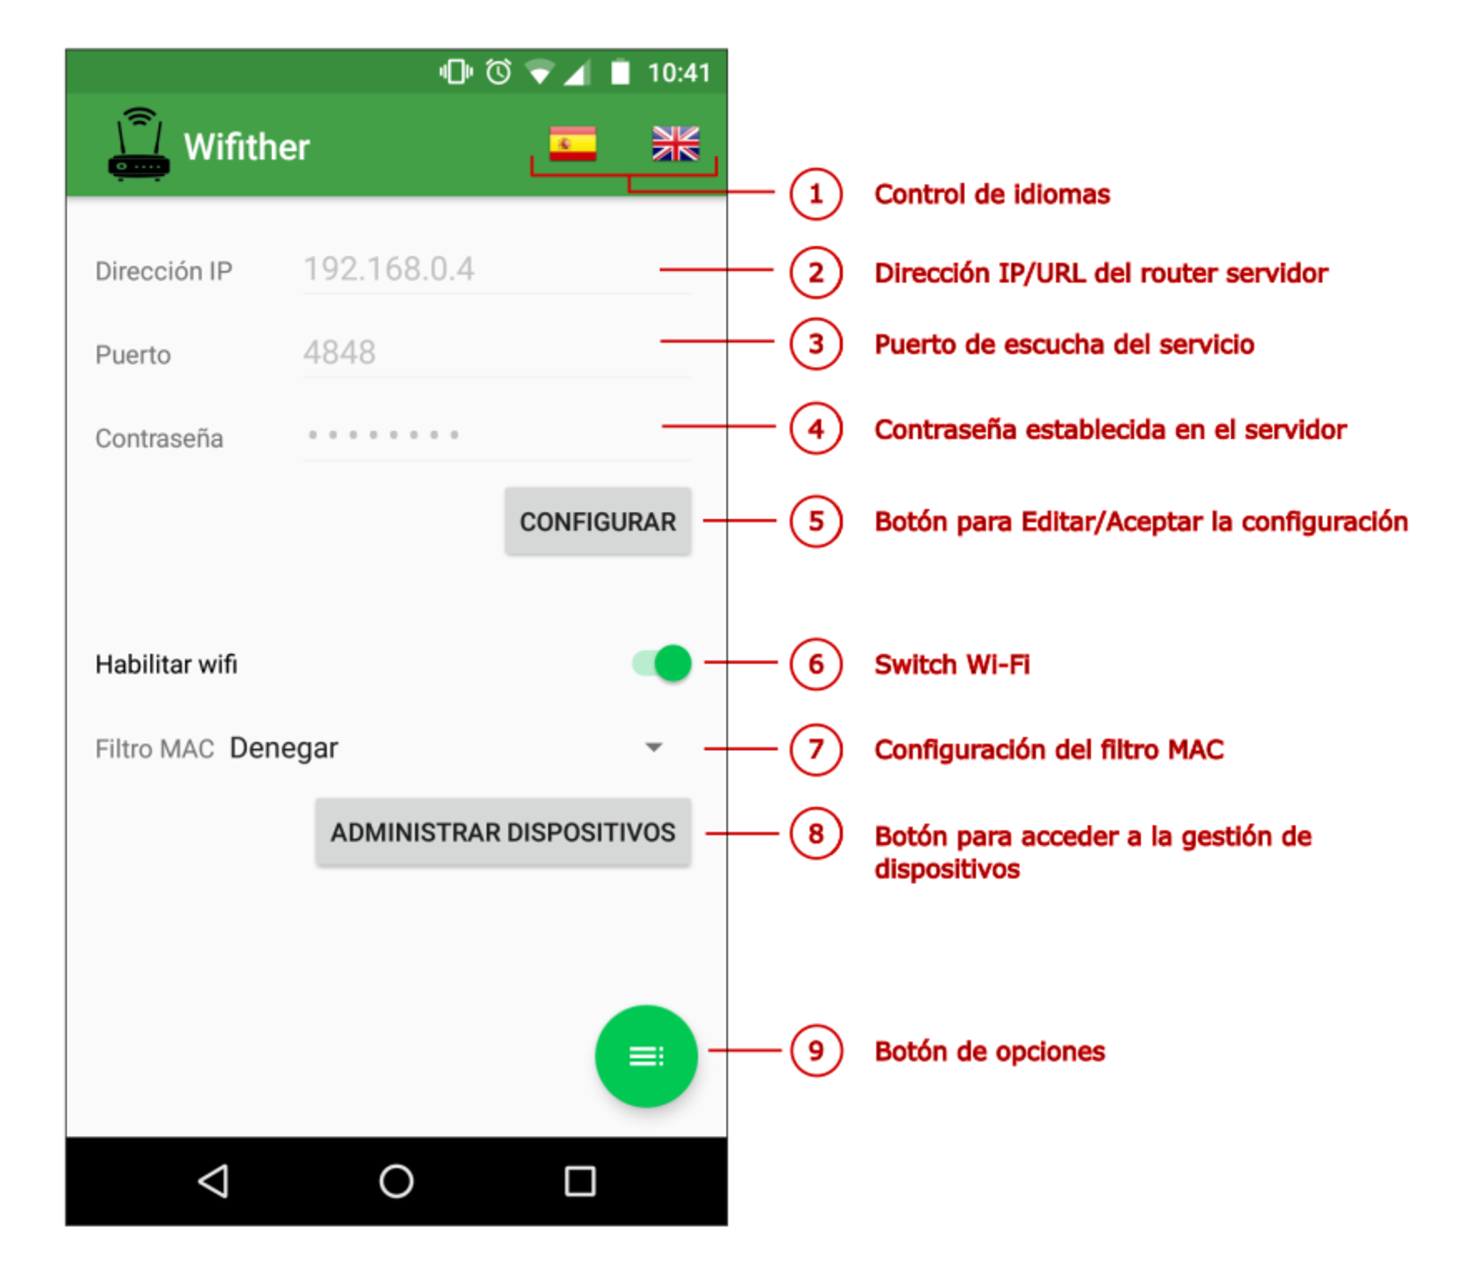
\includegraphics[scale=0.5]{main_activity_manual.eps}
            \caption*{Pantalla principal}
            \label{fig:main_activity_manual}
    \end{figure}

    \todo{Y la organización de esto???}
    \begin{figure}[h!]
        \centering
            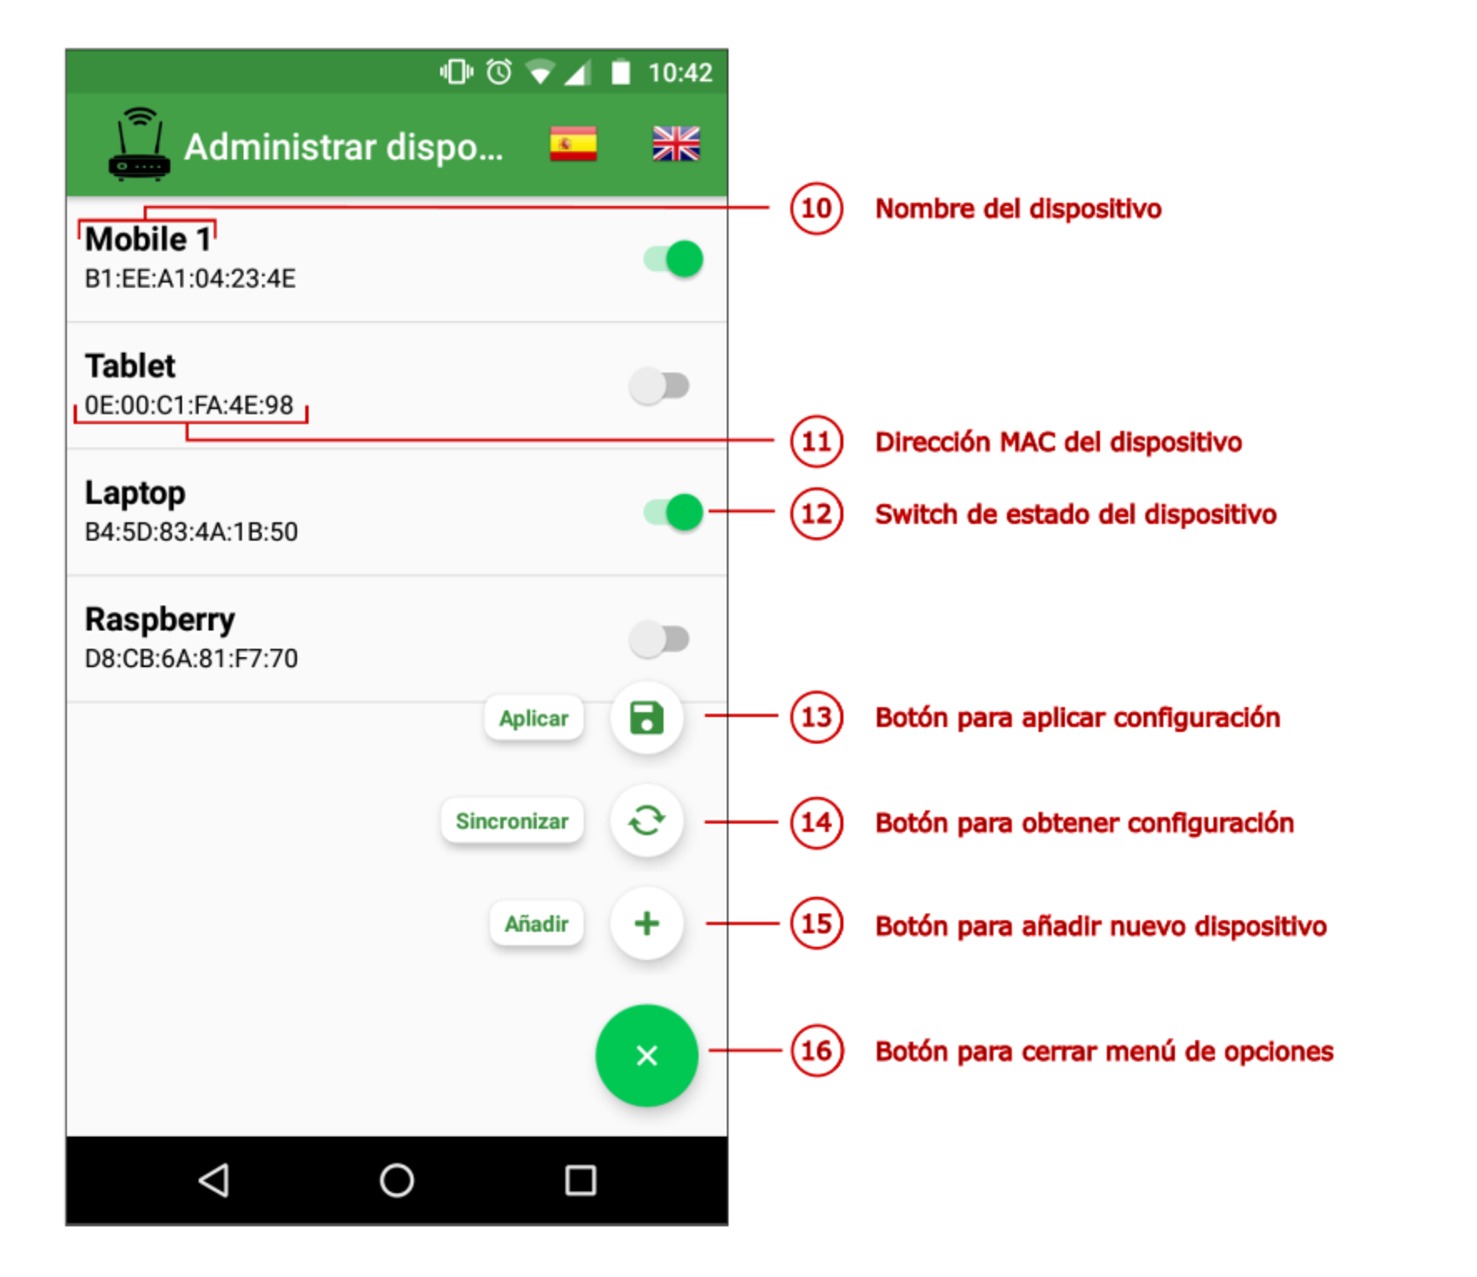
\includegraphics[scale=0.5]{devices_activity_manual.eps}
            \caption*{Administración de dispositivos}
            \label{fig:devices_activity_manual}
    \end{figure}

    \todo{enumerar}

    1. Control de idiomas
    Permite seleccionar el idioma con el que se muestran las opciones de la interfaz de usuario, están disponibles castellano e inglés, el idioma por defecto de la aplicación es el inglés.

    2. Dirección IP/URL del rputer servidor
    Es el campo de texto donde se especifica la dirección del router OpenWRT en el cual se ha instalado la aplicación y sobre el que se desea gestionar la red Wi-Fi. La edición de este campo está deshabilitada por defecto, para cambiar su contenido se debe hacer uso del botón señalado con el número 5 en la \ref{fig:main_activity_manual}

    3. Puerto de escucha del servicio
    Es el puerto que se indica al iniciar la aplicación en el router OpenWRT y que se utiliza para recibir las órdenes desde el dispositivo móvil. La edición de este campo está deshabilitada por defecto, para cambiar su contenido se debe hacer uso del botón señalado con el número 5 en la \ref{fig:main_activity_manual}

    4. Contraseña establecida en el servidor
    Es la contraseña que se indica al iniciar la aplicación en el router OpenWRT y que se utiliza para encriptar y desencriptar las órdenes enviadas desde el dispositivo móvil. La contraseña debe contener al menos ocho caracteres. La edición de este campo está deshabilitada por defecto, para cambiar su contenido se debe hacer uso del botón señalado con el número 5 en la \ref{fig:main_activity_manual}

    5. Botón para Editar/Aceptar la configuración
    Este botón habilita la edición de los campos de configuración señalados con los números 1, 2 y 3 en la \ref{fig:main_activity_manual}. Tras ser pulsado, el texto del botón cambia a \textit{Confirmar}, y debe ser pulsado para guardar la nueva configuración.

    6. Switch Wi-Fi
    Enciende o apaga la red Wi-Fi en el router OpenWRT, la posición iquierda indica que la red Wi-Fi está apagada, la posición hacia la derecha indica que está encendida.

    7. Configuración del filtro MAC
    Permite seleccionar la configuración del filtro MAC en el router OpenWRT. El selector tiene tres posiciones: \textit{Deshabilitado}, \textit{Permitir} y \textit{Denegar}.
    Si el filtro MAC está deshabilitado, cualquier dispositivo puede conectarse a la red Wi-Fi sin restricción de ningún tipo.
    Si el filtro MAC está configurado para \textit{Permitir}, significa que sólo pueden acceder a la red Wi-Fi los dispositivos que hayan sido especificados para que el filtro les sea aplicado.
    Si el filtro MAC está configurado para \textit{Denegar}, significa que tienen acceso a la red todos los dispositivos excepto los especificados para que el filtro les sea aplicado.

    8. Botón para acceder a la gestión de dispositivos
    Al pulsarlo se accede a un nuevo conjunto de opciones desde donde se pueden adicionar, editar y eliminar dispositivos, además de poder seleccionar los dispositivos con los que se desea aplicar el filtro MAC.

    9. Botón de opciones
    Permite acceder a las opciones marcadas con los puntos 12, 14 y 15 en la \ref{fig:devices_activity_manual}

    10. Nombre del dispositivo
    Es un indicador distintivo para cada dispositivo, es determinado por el usuario al añadir un nuevo dispositivo y es un campo obligatorio.

    11. Dirección MAC del dispositivo
    Identificador único del adaptador de red del dispositivo. Es especificado por el usuario al añadir un nuevo dispositivo y debe cumplir con un formato específico compuesto por seis pares de caracteres hexadecimales separados por dos puntos(:). Si el formato introducido no es correcto, el botón \textit{Añadir} queda deshabilitado.

    12. Switch de estado del dispositivo
    Añade o elimina dispositivos para que se le aplique la configuración del filtro MAC, la posición iquierda indica que la configuración del filtro NO se aplica al dispositivo, la posición hacia la derecha indica que la configuración del filtro SÍ se aplica al dispositivo.

    13. Botón para aplicar configuración
    Aplica en el router OpenWRT la configuración que haya sido establecida.

    14. Botón para optener configuración.
    Actualiza el dispositivo móvil con la configuración actual del router OpenWRT. Esta opción es útil cuando se gestiona la red desde más de un dispositivo móvil, de esta forma cada dispositivo puede saber siempre la última configuración aplicada en el router.

    15. Botón para añadir nuevo dispositivo
    Muestra un cuadro de diálogo que permite introducir los datos del nuevo dispositivo y añadirlo a la lista de dispositivos

    16. Botón para cerrar el menú de opciones
    Cierra el menú de opciones, también puede ser cerrado presionando sobre cualquier espacio fuera del menú.

    \todo{subsection??}
    Para editar la información de un dispositivo, mantener pulsado sobre el mismo hasta que aparezca un cuadro de diálogo y seleccionar la opción editar. La información del dispositivo debe cumplir los siguientes requisitos: El nombre de dispositivo no puede estar vacío, y la dirección MAC debe estar compuesta por seis pares de caracteres hexadecimales separados por dos puntos(:)

    Para editar la información de un dispositivo, mantener pulsado sobre el mismo hasta que aparezca un cuadro de diálogo y seleccionar la opción eliminar.

    \textbf{IMPORTANTE:} Debe tenerse en cuenta que una mala configuración del filtro MAC puede provocar la pérdida de la conexión en el dispositivo desde el que se está gestionando la red Wi-Fi si está directamente conectado a esta. La configración establecida debe ser revisada cautelosamente antes de ser aplicada. En caso de pérdida de conexión por este motivo, contactar con el encargado/a de instalar y configrar la aplicación en el router OpenWRT.

\section{Conclusiones y trabajo futuro}


    \subsection{Principales aportaciones}

    % deberanse destacar entre 3 e 5 aportacións importantes do

    % traballo realizado, tendo en conta os obxectivos fixados.


    \subsection{Conclusiones}

    % incluiranse todas as conclusións de tipo técnico e persoal.


    \subsection{Trabajo futuro}
    % presentaranse posible ampliacións e traballos relacionados por facer.


\section{Referencias}
``I always thought something was fundamentally wrong with the universe'' \citep{adams1995hitchhiker}
% deberanse citar todas as fontes de información empregadas para a realización do traballo.

% 1. Autor/a/es/as.

% 2. Título do artigo, libro, monografía,...

% 3. Editorial ou nome da revista.

% 4. Número da revista, volume e páxinas (só para revistas).

% 5. Ano de publicación.

% 6. Dirección e data de consulta (só para URL).

% Recoméndase empregar para referencias de artigos, revistas, e outras fontes de

% referencia, o formato APA, ISO 690, IEEE ou similares, e uniformizados ao longo de

% toda a sección.

% Deberase empregar un estilo uniforme para todas elas e aportarase, en cada caso:

\section{Anexos}

% incluiranse outros elementos de interese no TFG que se consideren necesarios para a

% mellor comprensión do mesmo.

\section{Tecnologías}
\todo{debería empezar por "Es tal cosa" siempre o meejor empezar con el nombre, o sin nada?}
    \subsection{OpenWRT}
        OpenWRT es una distribución Linux para dispositivos embebidos\todo{y routers}. En lugar de existir como un firmware estático, OpenWRT proporciona un sistema de archivos totalente modificable con gestión de paquetes, el cuál permite sustituir el sistema del proveedor y una mayor personalización del dispsitvo. Es el framework perfecto para el desarrollo de una aplicación sin tener que construir todo el firmware que a rodee.

    \subsection{C}
        Es un lenguaje de programación imperativo de prósito general que destaca por la eficiencia de su código y su popularidad para crear software de sistemas debido a su flexibiliadad y control a muy bajo nivel. Es la opción ideal cuando se desea ahorrar la mayor cantidad de espacio posible en la construcción del software, necesidad común de dispositivos embebidos. \todo{solo embebidos?}

        \subsubsection{OpenWRT SDK}
            El SDK es un conjunto de herramientas de programación reubicables y precompiladas que permiten la compilación cruzada de paquetes para el espacio de usuario de OpenWRT\todo{ref openwrt} sin tener que compilar todo el sistema desde cero.

        \subsubsection{uClibc}
            \todo{yewClibc}
            Es una librería \todo{en?}C para el desarrollo de sistemas Linux embebidos, es más pequeña que la librería \todo{poner estilo} glibc (GNU C Library) y soporta prácticamente todas las aplicaciones que son desarrolladas con esta. uClibc \todo{yewClibc} es capaz de gestionar librerías compartidas e hilos, además de funcionar con procesadores de varias arquitectura, entre las que se incluyen amd64, ARM, mips/mipsel, alpha, PowerPC y SH.

        \subsubsection{OpenSSL}
            Es un proyecto de código abierto que implementa la una librería criptográfica de propósito general. Provee un conjuto de herramientas robusto, de nivel comercial, para los protocolos SSL/TLS.

    \subsection{OpenVPN}
        \todo{openvpn}

    \subsection{sed}
        Es una utilidad unix, un editor de flujo capaz de analizar y transformar textos utilizando un simple y compacto lenguaje de programación. Permite el uso de expresiones regulares y tratamiento de archivos con un gran número de líneas de forma rápida.

    \subsection{\LaTeX}\todo{debería ir así?}
        Es un sistema de tipografía de alta calidad, incluye mecanismos diseñados para la creación de documentación científica y técnica por lo que se ha convertido en el estándar de facto a la hora de desarrollar esta tarea. Está concebido como siftware libre, y cuenta con múltiples librerías que añaden funcionalidades comunmente necesarias para la creación de estos doumentos.

    \subsection{Java}
        Es un lenguaje de programación orientado a objetos, compilado, de propósito general y alto nivel. Es el principal lenguaje para el desarrollo de aplicaciones móviles Android, además de ser utilizado para soluciones web, cliente-servidor, sistemas distribuidos, etc.

    \subsection{Git}
        Es un sistema de control versiones distribuido diseñado para controlar proyectos de cualquier tamaño con rapidez y eficacia. Es de código abierto y ofrece medios para guardar, analizar y revertir cambios realizados en versiones actuales y anteriores, además del control de ramas que permite mantener y trabajar en más de una versión de un proyecto de forma simultánea.

\section{Herramientas} \todo{Herraminetas?}
    \todo{justificación de la utilización? no llega con explicar las caracterísiticas que lo distinguen?}
    \subsection{Atom}
        Es un editor de texto de código abierto desarrollado por GitHub Inc.,\todo{Qué hago aquí?} escrito en JavaScript, moderno, accesible y modificable en su totalidad. Es completamente personalizable, de forma que brinda el entorno de trabajo más cómodo y productivo posible, sin necesidad de modificar ningún archivo de configuración durante el desarrollo de proyectos. Cuenta con una muy amplia gama de paquetes, también de código abierto, que añaden y mejoran funcionalidades del editor.

    \subsection{Visual Studio Code}
        Es una herramienta desarrollada por Microsoft que combina las simplicidad de un editor de texto con lo que necesitan los desarrolladores para su ciclo básico "edit-build-debug" \todo{style}. Visual Studio Code provee soporte exhaustivo para la creación y depuración de código, además de un modelo extendible y una integración de bajo consumo de recursos con las herramientas existentes.

    \subsection{TeX Live}
        Es un una distribución libre para los sistemas de tipografía TeX\todo{ref latex}. Está disponible para Linux y Windows incluyendo la mayoría de programas, micro paquetes y fuentes que son software libre. Actualmente es la distribución por defecto de esta tecnología en múltiples distribuciones Linux como openSUSE, Fedora, Debian, Ubuntu y Gentoo, además de ofrecer soporte para múltiples idiomas.

    \subsection{Android Studio}
        Es el \todo{estilo}IDE (Integrated development environment) oficial para la creación aplicaciones Android. Ofrece herramientas para la edición de códigos de primer nivel, depuración, control de rendimiento y compilación instantánea. \todo{releer}Provee de un emulador Android que permite comprobar el funcionamiento del código de forma rápida y brinda un conjunto de opciones dinámicamente configurables en cuanto a tamaño, prestaciones y control de sensores. Posee integración condiferentes sitemas actuales y cuenta con soporte para librerías externas configurables para su compilación junto con la aplicación.

    \subsection{GitHub}
        Es una plataforma colaborativa de control de vesiones online basada en Git\todo{ref git} y desarrollada por GitHub Inc. Ofrece todas las funcionalidades de gestión de códigos que ofrece Git\todo{ref git} así como sus propias características basadas en la web. Provee control de acceso y varias opciones colaborativas como el control de errores, petición de funcionalidades, gestión de tareas y wikis. La plataforma cuenta con un servicio de pago que permite la creación de repositorios privados, este servicio está disponible de forma gratuita junto a un conjunto de herramientas de desarrollo que la empresa ofrece en un paquete para estudiantes verificados.

    \subsection{Lucidchart}
        Es una aplicación online enfocada a la creación de diagramas profesionales desde una interfaz web. Es una herramienta realmente cómoda a la hora de documentar proyectos grandes debido a lo sencillo y amigable de su entorno. Además, brinda integración con diferentes aplicaciones externas como Dropbox, Slack y Microsoft Office. 

    \subsection{Inkscape}
        Es un editor profesional de gráficos vectoriales disponible para Windows, Mac OS X y Linux. Es de código abierto y soporta una gran variedad de formatos, entre los que se incluye \textit{.eps}, el formato utilizado por latex. Además brinda una amplia variedad de herramientas para realizar trazado vectorial, manipulación de objetos y edición de textos.
        \todo{revisar}

    \subsection{OpenVPN for Andorid}
    \todo{hacer}

\bibliographystyle{plain}
\bibliography{references}

\end{document}
